% !TEX root = ../main.tex

\chapter{Proof construction}
We will be using Circom to generate an arithmetic circuit, and SnarkJS for the proof generation.

\paragraph{Circom} is a domain-specific language designed for creating arithmetic circuits, specifically utilized in zk-SNARKs.
Within Circom, circuit code is written to define the desired constraints. One notable distinction from other languages is the utilization of signals and templates.
Templates can be conceptualized as functions that operate as circuits. The primary template receives signals as inputs and produces other signals as outputs. Signals can be classified as either public or private.
Assigning a value to a signal contributes to the constraint system and the witness calculation process.
Input and outputs are signals, and you can have additionnal intermediate signals.
During circuit compilation, constraints are generated in r1cs format. Additionally, compiling a circuit produces a witness file containing the data essential for verifying the constraints and demonstrating the correct behavior of the circuit.


\paragraph{SnarkJS} is a JavaScript library that provides tools for working with zk-SNARKs, including circuit compilation.
SnarkJS facilitates generating zk-SNARK proofs for specific instances of the circuit using the r1cs and witness file.
SnarkJS also provides utilities for verifying the proofs.


\section{Proof of liabilities}
\label{subsec:pl}
The proof of liabilities operates on a list of balances and a list of email hashes as private inputs.
The first purpose of the circuit is to validate that all values are non-negative and that all balances fall within a specified range.
These verifications are crucial to prevent overflow or underflow issues, given that the operations occur within a finite field.

Subsequently, the proof of liabilities constructs a Merkle tree and outputs the total balance sum and the root hash of the Merkle tree.
The pseudocode for the circuit is found \hyperref[subsec:plc]{here}.

\paragraph{Inputs}
\begin{itemize}
   \item List of balance (private)
   \item List of email hash (private)
   \end{itemize}

\paragraph{Outputs}
\begin{itemize}
   \item Balance Sum 
   \item Root hash
   \item No negative values - boolean
   \item All small range - boolean
   \end{itemize}

This proof of liabilities operates as intended because it returns the sum of the liabilities, which is exact because of the verifications.
It also returns the root hash, ensuring you cannot alter any values inside the merkle tree. The merkle tree is hidden so that we do not
give any information about users and their balances.
The root hash will be used to verify the inclusion of the balances.

In a complete proof of reserves, the balance sum would be a private output. We would have another circuit proving that the sum of liabilities is smaller
than the sum of assets, without revealing the balance.

\section{Proof of inclusion}
\label{subsec:pi}
The proof of inclusion aims to prove that the balance of a user is included in the Merkle Tree created in the proof of liabilities.
To prove that a balance is included, it is sufficient to show that you know the Merkle path of a user balance,
which we define using the list of neighbors sum, hash and binary.
The neighbors binary variable indicates whether the neighbor is on the left or the right.
The root hash, root sum, user balance and user email hash are public because it needs to be shown which user is in which tree.

For the next figure, the blue nodes represent the value of the merkle path.
We would have $neighborsSum=[29,61]$, $neigborsHash=[Hash(User1),Hash(L2,R2)]$ and $neighborsBinary=[0,1]$.
\begin{figure}[H]
   \centering
   \includegraphics[width=130mm]{MerklePath.png}
   \caption{Merkle Path}
   \label{overflow}
   \end{figure}


\paragraph{Inputs}
\begin{itemize}
   \item List of neighbors sum (private)
   \item List of neighbors hash (private)
   \item List of neighbors binary (private)
   \item Root hash (public)
   \item Root sum (public)
   \item User balance (public)
   \item User email hash (public)
   \end{itemize}


\paragraph{Outputs}
\begin{itemize}
   \item Balance included - boolean
   \end{itemize}

\paragraph{}
In the \hyperref[subsec:pic]{circuit}, we verify that the combination of the user balance, sum and merkle path gives the right root hash and root sum. There is no additional
verifications since they are already done for this root hash, in the proof of liabilities.

\section{Daily proof of liabilities}
We aim to enhance our current \hyperref[subsec:pl]{circuit} by minimizing the work needed in subsequent rounds.
The first thing to explore is recursion proofs, as they were specifically created to reduce the total computational effort across rounds.

\subsection{Aggregation proofs}
The main advantage of the aggregation proof is in streamlining the verification process. For instance, in the second round, we can prove the integrity of the current round and all previous rounds.
However, this benefit comes with trade-offs. The first drawback is the increase in proof size, as it necessitates to prove the current circuit and verify the previous ones.
When considering the frequency of verification, having a fixed number of nodes verify the proof daily, it would be illogical to make the nodes verify the previous rounds every single day.
On the other hand, if the verification is not consistent, or there is a need for new nodes to be able to come in and verify every proof quickly, then aggregation becomes more appealing.

In our case, the priority is to produce daily succinct proofs. We need to ensure the integrity of every round, while keeping the proof size to a minimum.
Therefore, having our nodes verify the circuit at every round without the computational overhead of the aggregated proof is sufficient.

\subsection{Other recursion proofs}
The aggregation proof stands out as the only recursion proof potentially useful in certain scenarios.
If we examine the other types of recursion proofs, namely Recursion scheme, accumulation and Folding scheme, they all have one thing in common.
They are all designed to verify multiple rounds concurrently.
This approach is not aligned with our objectives. We are interested in working on rounds independently and reducing the individual workload.

\subsection{Change circuit}
If we cannot use any recursion schemes, we need an alternative approach to reduce the complexity of subsequent rounds.
Our solution is to reutilize the same Merkle Tree as the previous rounds, modify  and adapt it to include the changes.
The key challenge is that the Merkle Tree was built inside the circuit, and is therefore not accessible.

What we will be doing, in our modified circuit, is adjust the Merkle Tree inside the circuit.
For every change, we send the corresponding Merkle Path which will be verified by the circuit.
The circuit will then compute a new Root Hash for each change and output the final Markle Hash.

The standard verification will be applied to the new values (e.g., non-negative values, limited range).

\paragraph{Inputs}
\begin{itemize}
   \item List of old email hash (private) - 1 per change
   \item List of old values (private) - 1 per change
   \item List of new email hash (private) - 1 per change
   \item List of new values (private) - 1 per change
   \item List of temporary root hash (private) - 1 per change
   \item List of temporary root sum (private) - 1 per change
   \item Old root hash (public)
   \item Old root sum (public)
   \item List of neighbors sum (private) - 1 list per change
   \item List of neighbors hash (private) - 1 list per change
   \item List of neighbors binary (private) - 1 list per change
\end{itemize}

\paragraph{Outputs}
\begin{itemize}
   \item Valid hash
   \item Valid sum
   \item No negative values
   \item All small range
   \item New root hash 
   \item New root sum
   \end{itemize}

Here is an example of a change. In this case the change is a change in balance. First we prove that the 10 BTC of user 1 are 
included in the merkle tree. Then we prove that the 11 BTC of user 1 are included in the new merkle tree. After the last change we are left
with the new root balance and the new root hash. Not that for every change we only need 1 merkle path.

\begin{figure}
   \hfill
   \subfloat[Pre change]{\includegraphics[width=70mm]{MerklePath.png}}
   \hfill
   \subfloat[Post change]{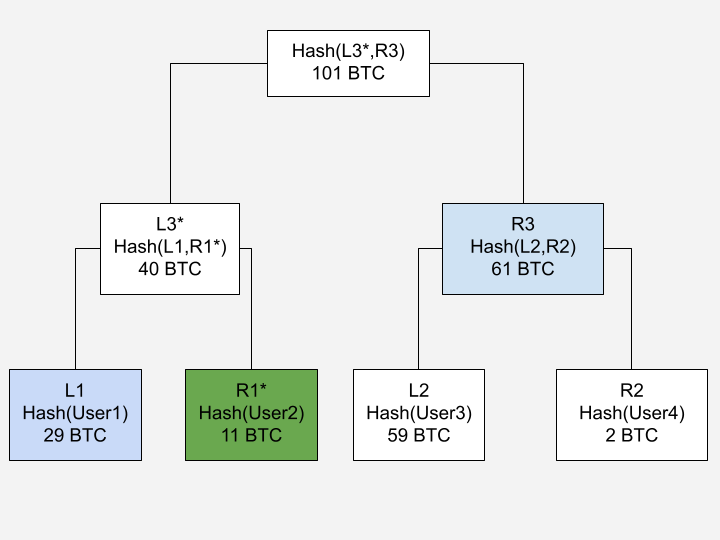
\includegraphics[width=70mm]{MerklePathTemp.png}}
   \hfill
   \caption{Merkle Tree change}
   \end{figure}


For every change in the merkle tree, we have the merkle path with the old values, the new values, the temporary root hash and
the temporary root sum.
The \hyperref[subsec:plcc]{circuit} is iterating over the changes and gives a final root hash and final root sum.

\subsubsection{Minimizing the number of changes}
To minimize the number of constraints, we want to minimize the number of changes.
We define a change as a hash change at the leaf level. Any new user, balance change or removal of old user is considered as a change.
The naive change calculation would be $changes = balanceChanges + newUsers + deprecateUser$.
However, a new user can take the node of a deprecater user. So we would have the equation $changes = balanceChanges +max(newUsers + deprecateUser)$.

\subsubsection{Constraint analysis}
Theorically, the new circuit makes sense. It should be quite faster than the original one, so let's analyze it.
We want to compare the number of constaints for the original circuit with the number of constraints with the change circuit.
The first assumption we are gonna need to do, is to assume the number of changes in a day. A completely arbitrary value would be $1\%$.
\begin{figure}[H]
   \centering
   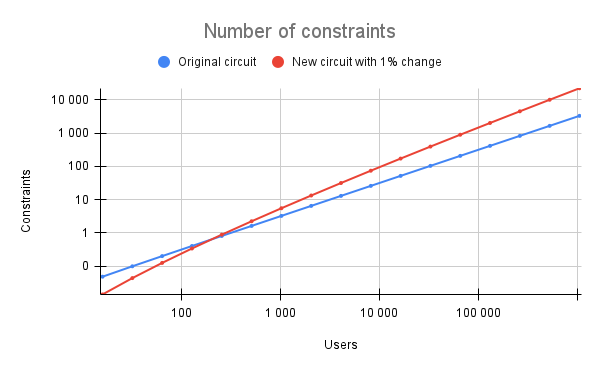
\includegraphics[width=130mm]{Number of constraints.png}
   \caption{Number of constraints original circuit vs new circuit with 1\% change}
   \label{overflow}
   \end{figure}
Once you reach more than 128 users with $1\%$ change, it is not worth it to use the new circuit. 
This is not really practical because any marketplace will have more than 128 users.
However, we can see that the number of constraints of the new circuit grows linearly for the number of change.
This means that two circuits of 0.5\% change would have a similar number of constraints as the one circuit with 1\% change.
We can take this a step further, and instead of looking at daily proof look at hourly proof.
Going with the assumption that $1\%$ change daily, we will assume that $0.05\%$ of the balances changes hourly.
Lets look at the number of constraints if $0.05\%$ of users change every hour.
\begin{figure}[H]
   \centering
   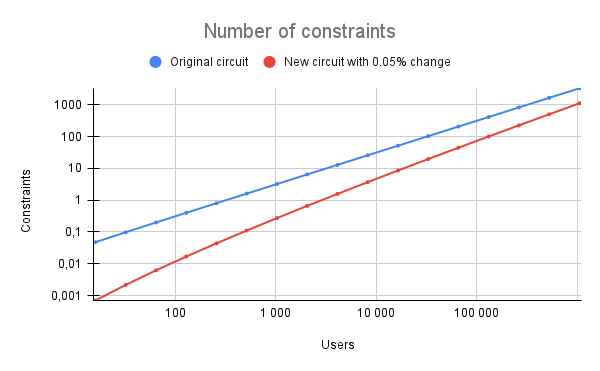
\includegraphics[width=130mm]{Number of constraints .05.png}
   \caption{Number of constraints original circuit vs new circuit with 0.05\% change}
   \label{overflow}
   \end{figure}
Even with more than 1 million users, there is still 3 times less constraints with our new circuit.
So if we want to do an hourly proof, it is less expensive with the new circuit than the old circuit.
We can take this a step further, and do a proof at every new block. We could have a merkle tree up to date for the liabilities side at every single block.

While the hourly proof and block proof is better with the new circuit, maybe a daily proof is sufficient for most use cases.
It is still less work to do the daily proof with the original circuit, than to do 24 hourly proof with the new circuit.

\section{Daily proof of inclusion}

Because a marketplace can have millions of users, it is impractical to build a proof of inclusion for every single user on a daily basis.
It is the user's responsibility to request a proof that their balance is included in the published Merkle tree.

In an ideal world, a Merkle tree would be published at least daily. However, it is once again impractical to require every user to verify their inclusion everyday.
Nevertheless, each user verifying its inclusion in the tree increases the chance that the proof of liabilities is valid and includes every single balance.
This is why it is primordial to find a way to make it easier to verify the inclusion. This is where Nova folding schemes come in.

The novel way to do proof of inclusion is to generate a proof of inclusion that is valid from the day of creation of the account, to the requested day by the user.
Normally you would need to create 500 different proofs for 500 days. However, we saw in the previous section that the nova folding scheme enables the 500 proofs into just one.
Verifying this one proof is the equivalent of verifying the 500, or any other number of days required.
This drastically simplifies the verification process.

Previously, when requesting a proof of inclusion, the user would only receive proof that their balance is included in the latest published Merkle tree. Now, the proof verifies that the balance has been included in every previously published Merkle tree.
This ensures that any malicious entity would be unable to alter ownership of balances across multiple days. It might seem like a small detail, but it is the detail that makes all the difference, and here is why.

In this chart, we can observe the failure probability, which represents the likelihood that a dishonest prover gets away with misbehaving.
If we take for example the orange line, where an exchange has 1 million users, we notice that the failure probability approaches 0 when over $4\%$ of users perform their verifications.
However, without utilizing folding, this principle doesn't extend to every round. It implies that for each round, we require a minimum of $4\%$ of users to have a proof with significant confidence.

\begin{figure}[H]
   \centering
   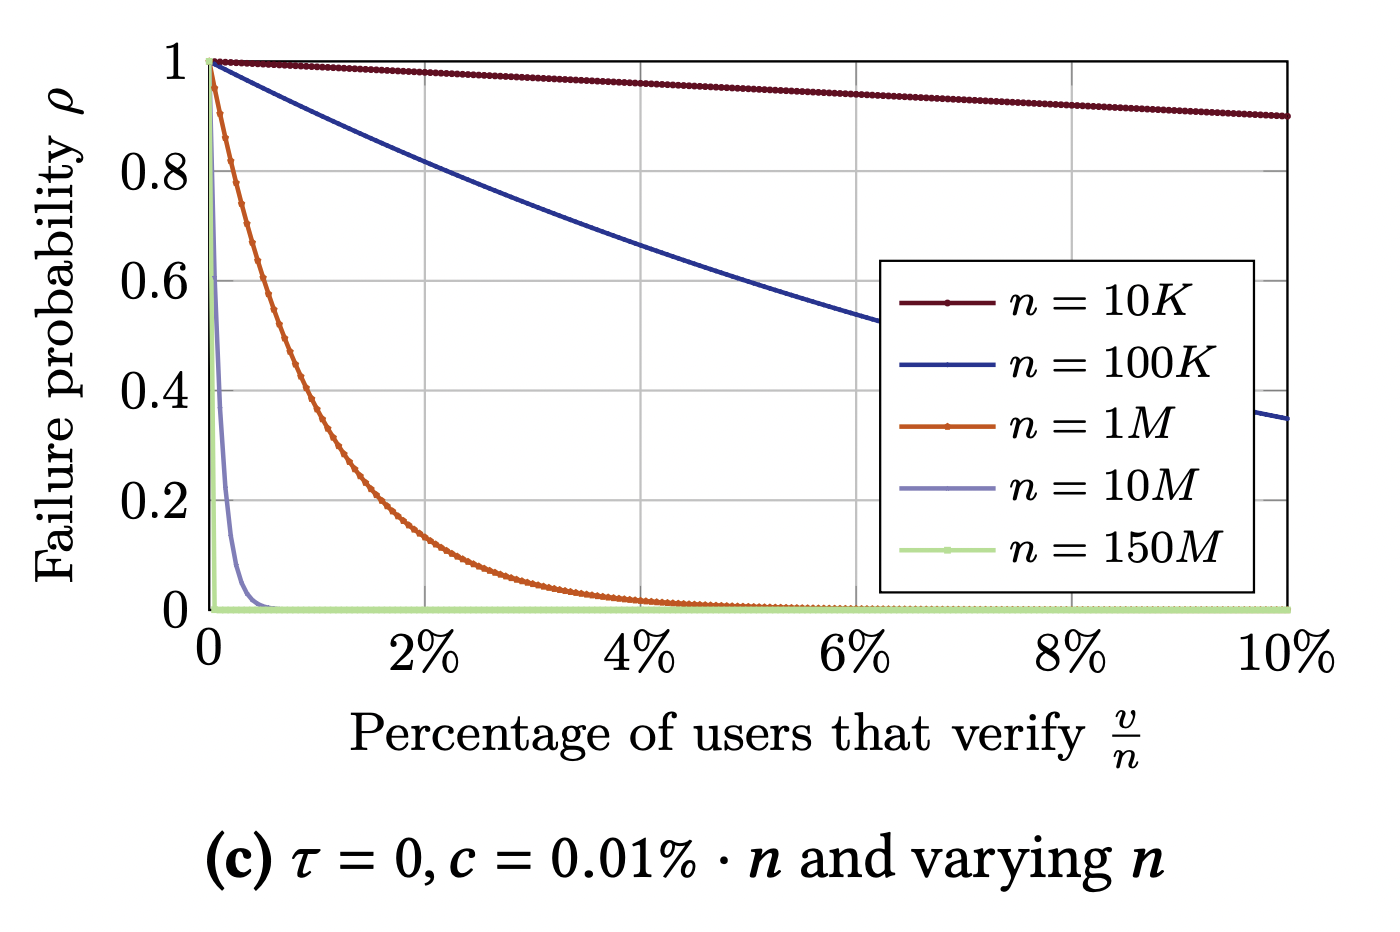
\includegraphics[width=130mm]{FailureProbability.png}
   \caption{Failure Probability \cite{GP21}}
   \label{overflow}
   \end{figure}

Now, lets evaluate the failure probability if we are using folding.
In the initial round, with no changes, the failure probability for 20k users remains at $13\%$.

\begin{figure}[H]
   \centering
   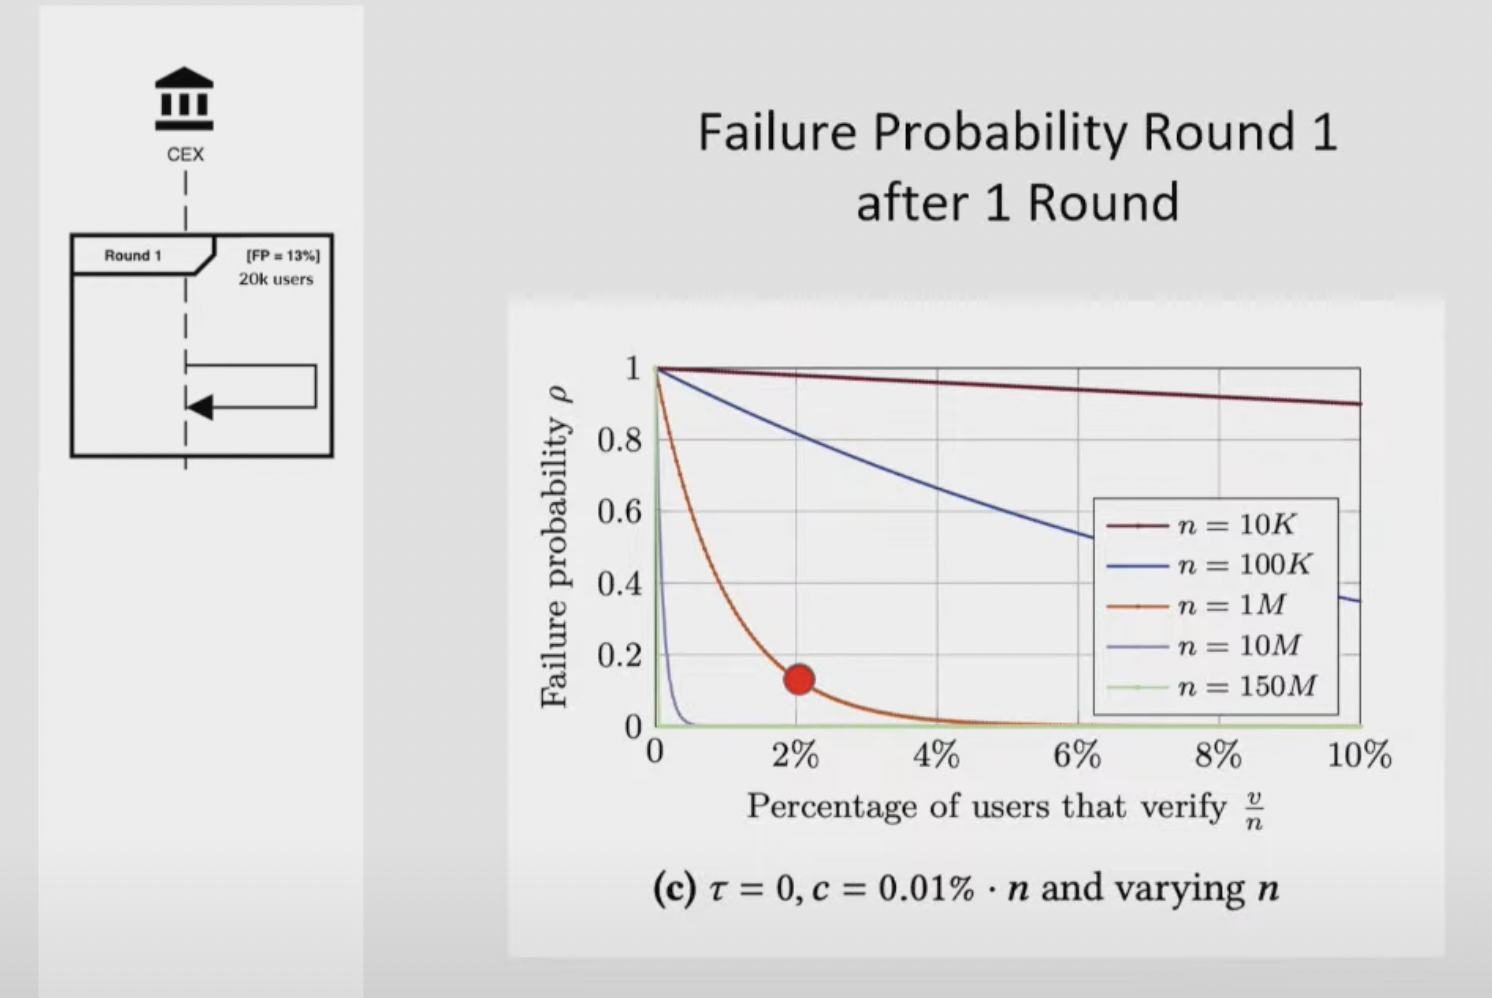
\includegraphics[width=130mm]{FailureProbabilityRound1.png}
   \caption{Failure Probability Round 1 \cite{NS23}}
   \label{overflow}
   \end{figure}

However, if we have 20k distinct users in round 2, the failure probability of round 1 decreases to $1.6\%$ .

\begin{figure}[H]
   \centering
   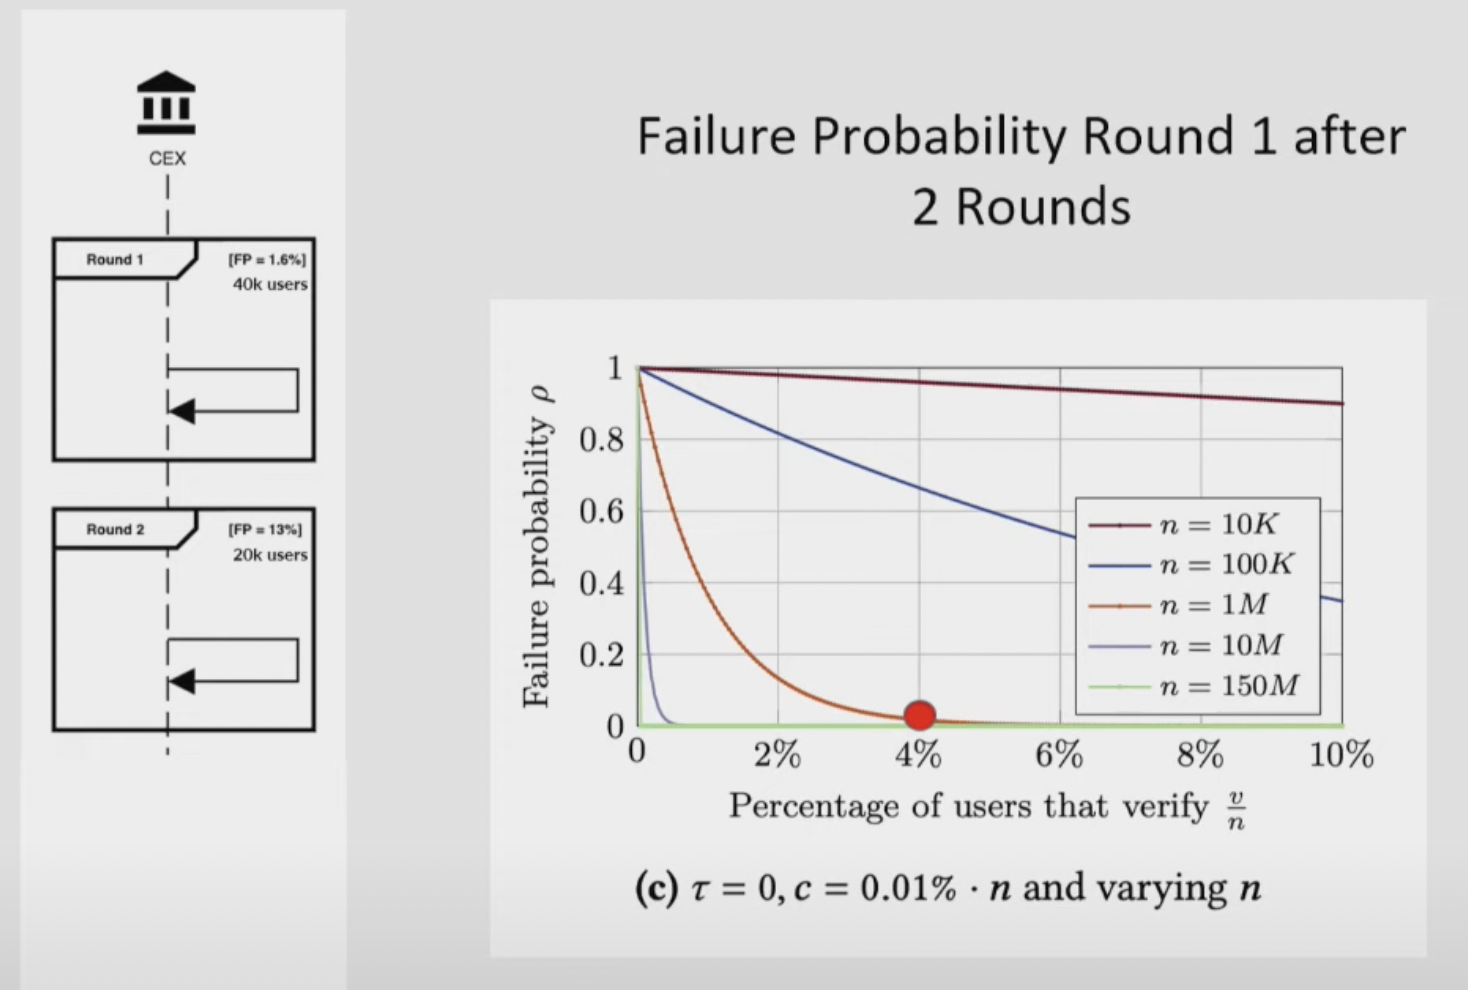
\includegraphics[width=130mm]{FailureProbabilityRound2.png}
   \caption{Failure Probability Round 1 After 2 Rounds\cite{NS23}}
   \label{overflow}
   \end{figure}

If we have 20k different users in round 3, the failure probability of round 1 further decreases to $0.2\%$ .

\begin{figure}[H]
   \centering
   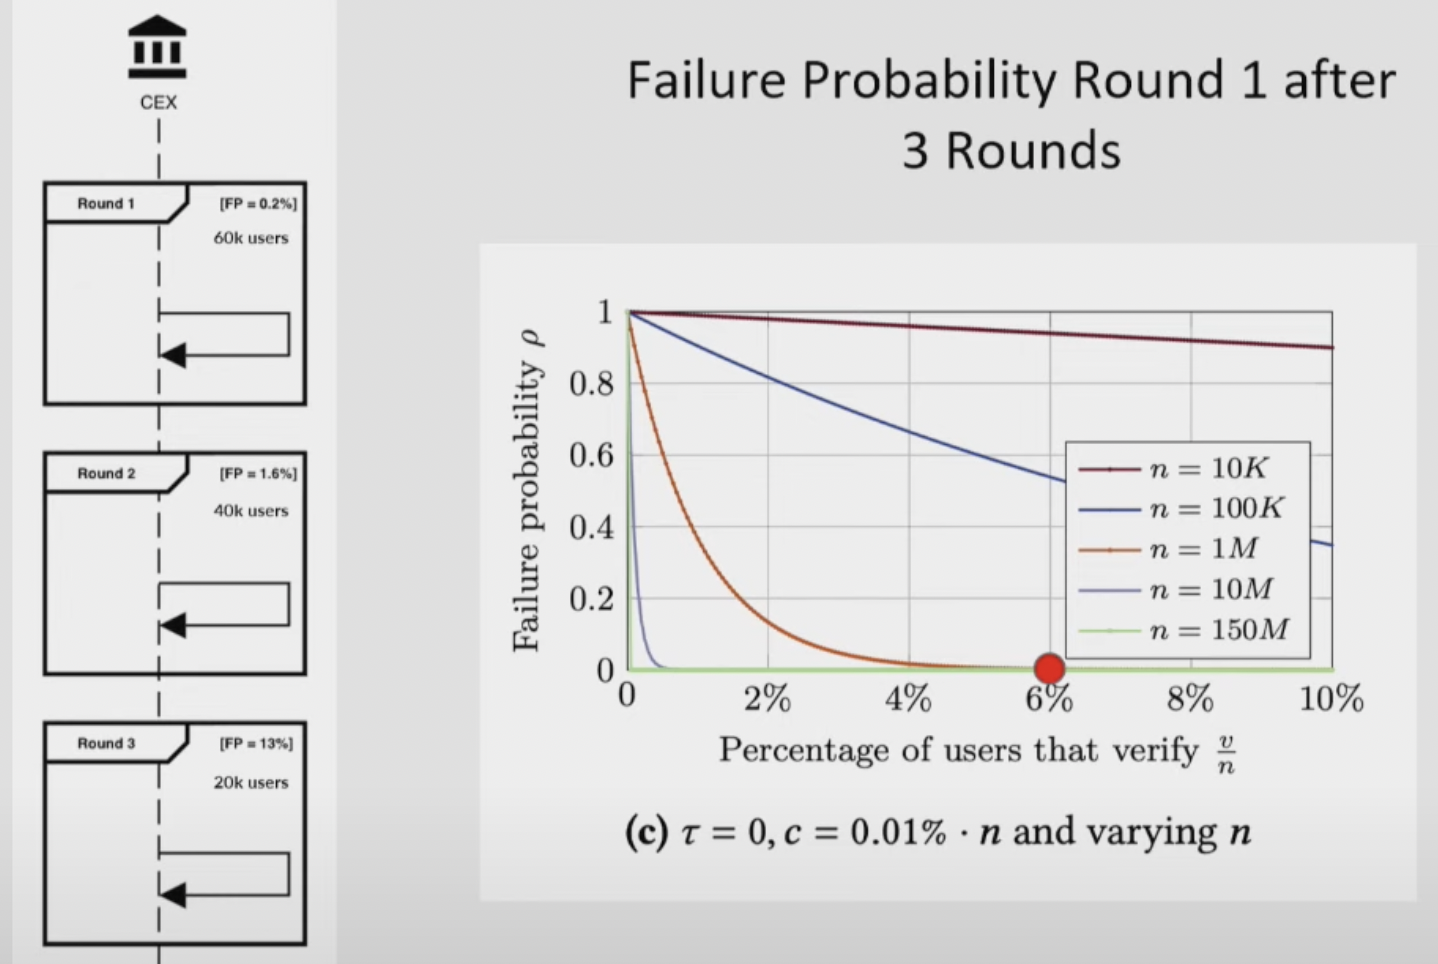
\includegraphics[width=130mm]{FailureProbabilityRound3.png}
   \caption{Failure Probability Round 1 after 3 Rounds \cite{NS23}}
   \label{overflow}
   \end{figure}
The key takeaway here is that without folding, you require $4\%$ of users to verify every round. However, with folding you only need
$4\%$  of users to participate in at least 1 round. This significantly reduces the burden on the user to verify, while increasing the confidence in the proof.

\subsection{Circuit Design}
The private inputs vary for each instance, whereas the public inputs are carried over from round to round.
In order to implement folding, we need to slightly adjust our \hyperref[subsec:pi]{circuit}. Everything except the way we handle inputs and outputs stays the same.
The private inputs vary for every instance, while the public inputs are carried over from round to round.

\paragraph{Inputs}
\begin{itemize}

   \item List of neighbors sum (private)
   \item List of neighbors hash (private)
   \item List of neighbors binary (private)
   \item Root hash (private)
   \item Root sum (private)
   \item User balance (private)
   \item User email hash (private)
   \item Steps in (public)
  
   \end{itemize}

\paragraph{Outputs}
\begin{itemize}
   \item Steps out (public)
   \end{itemize}

\paragraph{Steps}
\begin{itemize}
   \item Balance included
   \item Root sum
   \item Root hash
   \item User balance
   \item User email hash
   \end{itemize}

   All the data that is passed around between the circuits is public and is called step in and step out, and the regular inputs are private.
   The step in of a circuit is the step out of the previous one. 

\begin{figure}[H]
   \centering
   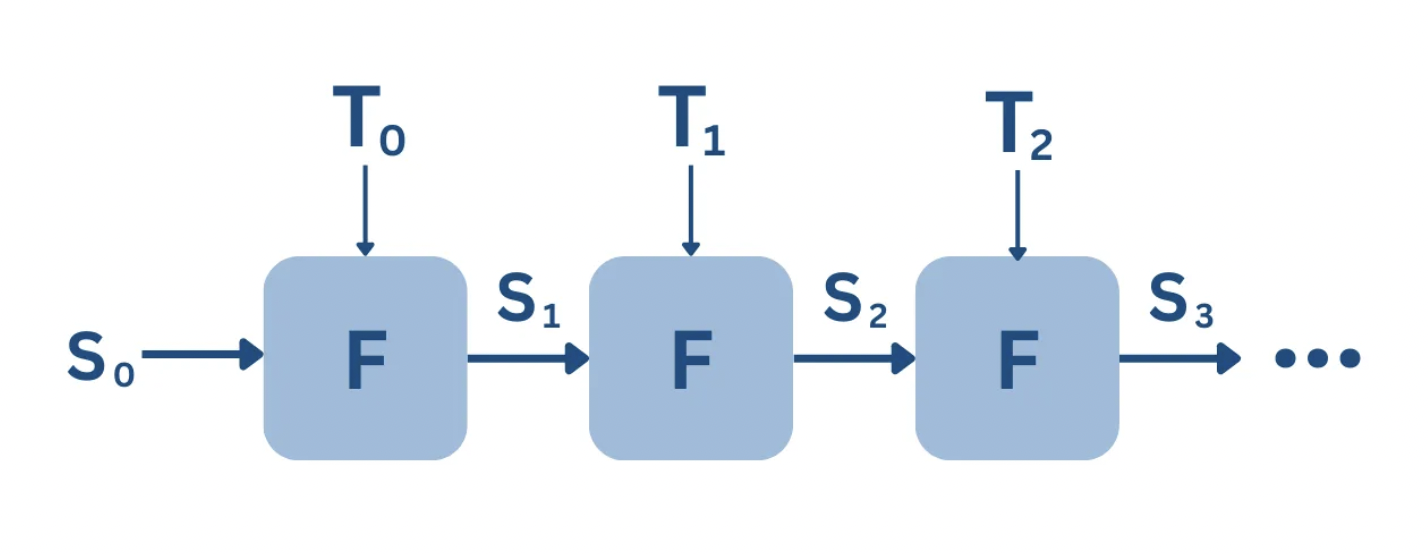
\includegraphics[width=130mm]{FoldingCircuit.png}
   \caption{Folding Circuit}
   \label{overflow}
   \end{figure}

S0 is the step in of the first change, S1 is the step out of first change and step in of second change. F is the folded circuit
and T is the number of time it is folded.

These steps encompass all the public values we initially had in the circuit.
None of the variables of the steps are used in the circuit itself. They are used as a means to make a value public.

The initial circuit takes meaningless values as inputs, while the following circuits take the public values of the previous circuit.
At the end you only have to verify a single proof. You also need to compare the circuit output with the proof of liabilities outputs for every round.

\section{Folded daily proof of liabilities}
With the original circuit, we saw how it was not usefull to use folding or any other recursion scheme.
However, with the new circuit we saw that we were able to separate a big proof into multiple smaller ones.
This aligns prefectly wth the recursions ideas.
We can separate our new circuit of $n$ changes into $m$ circuits, where $m <= n$, and fold the circuits together.

\begin{figure}[H]
   \centering
   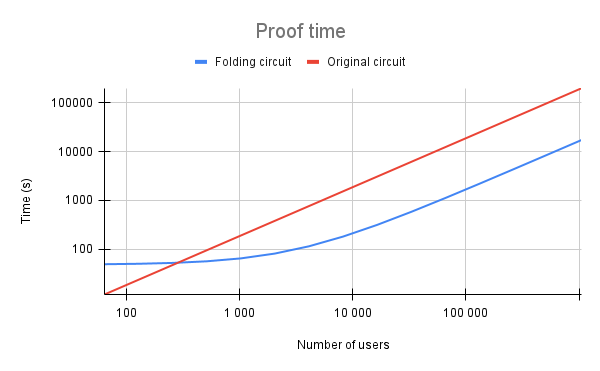
\includegraphics[width=130mm]{Proof time.png}
   \caption{Proof time original circuit vs folded circuit with 1\% change, 1 change by fold}
   \label{overflow}
   \end{figure}

As we can see, after 10 000 users, both circuits seems to be groing linearly, with the folded circuit doing much better. For instance,
at 1M users, we have the old circuit taking 196608 seconds, and the new circuits taking 17188 seconds. This is more than 10 times better.
We should take the number of seconds with a grain of salt, since these measurements were done on my mac, and there are much more performant computers out there.
The data we should focus on is that it took 10x less time for the folded circuit, and it was not event optimized. We were doing 1 change by circuit, so at 1M users we folded 10k circuits.

Now that we know that our circuit is better, we can optimize it.

\begin{figure}[H]
   \centering
   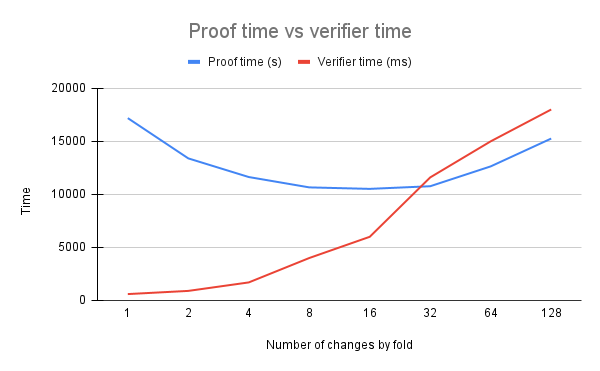
\includegraphics[width=130mm]{Proof time vs verifier time.png}
   \caption{Optimization of the proof time and verifier time of the folded circuit with 1\% change and 1M users}
   \label{overflow}
   \end{figure}

As we can see, the optimize time for the proofer, is between 8 and 32 changes by fold, while the verifier time seems to be groing at a monotonic pace.
Depending on the use case, you can decide the numbe of changes you should have for every fold. 

\subsection{Circuit design}
The folded change circuit is exactly the same as the regular change circuit, but the inputs works differently because some data is passed around the circuits.
There is 2 types of step variables; the variables needed in the following circuit, and the variables that are just there to be public. 
Starting from the inputs of the regular change circuit, the old hash and old sum root are moved to the step in, while all the outputs are moved to step out.

\paragraph{Inputs}
\begin{itemize}
   \item List of old email hash (private) - 1 per change
   \item List of old values (private) - 1 per change
   \item List of new email hash (private) - 1 per change
   \item List of new values (private) - 1 per change
   \item List of temporary root hash (private) - 1 per change
   \item List of temporary root sum (private) - 1 per change
   \item List of neighbors sum (private) - 1 list per change
   \item List of neighbors hash (private) - 1 list per change
   \item List of neighbors binary (private) - 1 list per change
   \item Step in (public)
   \end{itemize}

\paragraph{Outputs}
\begin{itemize}
   \item Steps out
   \end{itemize}

\paragraph{Steps}
\begin{itemize}
   \item Valid hash and valid sum
   \item No negative value and all small range
   \item Root hash
   \item Root sum
   \end{itemize}


%Mina proof of recursion
%summa
%https://summa.gitbook.io/summa/v/1/circuits/merkle-sum-tree-inclusion
%https://www.youtube.com/watch?v=sRAA1RYYHEs
%https://hackmd.io/@summa/HkGMF4Ovn#The-problem
